\documentclass[abstract=on,10pt,a4paper,bibliography=totocnumbered]{article}
\usepackage[paper=a4paper,left=35mm,right=35mm,top=25mm,bottom=30mm]{geometry}
\usepackage[doublespacing]{setspace}
\usepackage[english]{babel}
\usepackage[utf8]{inputenc}
\usepackage[round]{natbib}
\usepackage{amsmath}
\usepackage{colortbl}
\usepackage{amsfonts}
\usepackage{amssymb}
\usepackage{gensymb}
\usepackage{graphicx}
\usepackage{tikz}
\usepackage{enumerate}
\usepackage{enumitem}
\usepackage{subcaption}
\usepackage{booktabs}
\usepackage[hidelinks]{hyperref}
\usepackage[nameinlink]{cleveref}
% \usepackage{lineno}
\usepackage{multirow}
\usepackage{arydshln}
\usepackage[flushleft]{threeparttable}
\usepackage[nomarkers, nolists]{endfloat}
\usepackage[colorinlistoftodos]{todonotes}
\usepackage{scalerel}
\usepackage{tikz}
\usetikzlibrary{svg.path}

%------------------------------------------------------------------------------
%	Some Styling
%------------------------------------------------------------------------------
% Creating some TikZ styles
\tikzset{
  nonterminal/.style = {rectangle
    , minimum size = 6mm
    , very thick
    , draw = black!
  }
}

% Changing the style of captions in figures etc.
\captionsetup{labelfont=bf, format=plain, font=small}

% Change how equations are referenced
\renewcommand{\theequation}{Equation \arabic{equation}}%

% To be able to put an ORCID
\definecolor{orcidlogocol}{HTML}{A6CE39}
\tikzset{
  orcidlogo/.pic={
    \fill[orcidlogocol] svg{M256,128c0,70.7-57.3,128-128,128C57.3,256,0,198.7,0,128C0,57.3,57.3,0,128,0C198.7,0,256,57.3,256,128z};
    \fill[white] svg{M86.3,186.2H70.9V79.1h15.4v48.4V186.2z}
                 svg{M108.9,79.1h41.6c39.6,0,57,28.3,57,53.6c0,27.5-21.5,53.6-56.8,53.6h-41.8V79.1z M124.3,172.4h24.5c34.9,0,42.9-26.5,42.9-39.7c0-21.5-13.7-39.7-43.7-39.7h-23.7V172.4z}
                 svg{M88.7,56.8c0,5.5-4.5,10.1-10.1,10.1c-5.6,0-10.1-4.6-10.1-10.1c0-5.6,4.5-10.1,10.1-10.1C84.2,46.7,88.7,51.3,88.7,56.8z};
  }
}
\newcommand\orcid[1]{\href{https://orcid.org/#1}{\mbox{\scalerel*{

\begin{tikzpicture}[yscale=-1,transform shape]
  \pic{orcidlogo};
\end{tikzpicture}
}{|}}}}

%------------------------------------------------------------------------------
%	Titlepage: Header
%------------------------------------------------------------------------------
\title{Applying Step Selection Functions to Temporally Irregular GPS Data - A
Simulation Study}

% List of Authors
\author{
  David D. Hofmann\textsuperscript{1,2,\S} \orcid{0000-0003-3477-4365} \and
  Gabriele Cozzi\textsuperscript{1,2} \orcid{0000-0002-1744-1940} \and
  John W. McNutt\textsuperscript{2} \and
  Arpat Ozgul\textsuperscript{1} \orcid{0000-0001-7477-2642} \and
  Dominik M. Behr\textsuperscript{1,2} \orcid{0000-0001-7378-8538}
}

% Reduce spacing between authors
\makeatletter
\def\and{%
  \end{tabular}%
  \hskip -0.5em \@plus.17fil\relax
  \begin{tabular}[t]{c}}
\makeatother

% Current Date
% \date{\today}

% And here the masterpiece begins
\begin{document}

% Change page numbering
\pagenumbering{gobble}

% Required to be able to cite
\bibliographystyle{apalike}

% Create Titlepage
\maketitle

%------------------------------------------------------------------------------
%	Titlepage: Additional Info
%------------------------------------------------------------------------------
\begin{flushleft}

\vspace{0.5cm}

\textsuperscript{1} Department of Evolutionary Biology and Environmental
Studies, University of Zurich, Winterthurerstarsse 190, 8057 Zurich,
Switzerland.

\textsuperscript{2} Botswana Predator Conservation Program, Private Bag 13,
Maun, Botswana.

\textsuperscript{\S} Corresponding author (david.hofmann2@uzh.ch)

\vspace{4cm}

\textbf{Running Title:} None

\vspace{0.5cm}

\textbf{Keywords:} step selection analysis, gps data, animal movement, irregular
data

\end{flushleft}

%------------------------------------------------------------------------------
%	Abstract
%------------------------------------------------------------------------------
\newpage
\begin{abstract}
Animal movement data collected using GPS collars is often noisy and incomplete,
thus confronting movement ecologists with data that is not always uniformly
distributed in time. Step selection analysis has become a popular tool to use
such data and infer a species movement and habitat preferences. However, in
order to ensure comparability among steps, the method requires that consecutive
GPS relocations are collected at regular temporal intervals. To adhere to this
requirement, researchers typically discard large portions of their data and only
consider GPS bursts that were collected at similar intervals. Here, we assess
the appropriateness of this practice and use simulated data to examine if
including temporally irregular data could, in fact, improve estimates from
step-selection analyses. We also explore several alternative methods to account
for temporal irregularity. Our results suggest that utilizing a full dataset,
even if it contains temporal irregularities, improves the accuracy of step
selection estimates, especially when an appropriate method is chosen to account
for temporal irregularities.
\end{abstract}

%------------------------------------------------------------------------------
%	Main Text
%------------------------------------------------------------------------------
\newpage

\onehalfspacing
\tableofcontents
\doublespacing

% Change page numbering
\newpage
\pagenumbering{arabic}

% Create linenumbers
% \linenumbers

\section{Introduction}
Researchers usually collect GPS on fixed temporal intervals (could do a quick
and dirty analysis on MoveBank) ranging from a few minutes, to multiple hours or
even days between subsequent reolocations. Despite this, GPS devices frequently
fail to adhere to the anticipated schedule, for instance due to cloud cover,
thus resulting in GPS data with irregular temporal intervals. In some cases, the
GPS schedule may intentionally be subject to change to maximize battery
lifetime. For example, \cite{Cozzi.2020} increased the fixrate of their GPS
collars once per week from 4 to 8 fixes per day, aiming to collect more fine
scaled data for a limited time. In either case, the data at hand will be patchy
in terms of the temporal lag between consecutive recordings. We chose to coin
this type of data \textit{irregular}, because it is not collected on the
anticipated fixrate schedule and therefore not directly comparable to the vast
majority of the collected data.

Step selection analysis (SSA) is a powerful framework that enables researchers
to investigate the habitat and movement kernel of their focal species. While the
habitat kernel describes relative habitat preferences of the study species, the
movement kernel describes its movement patterns. SSA works by comparing spatial
covariates at locations where the studied animal has been observed, to a set of
locations where the animal was presumably absent. For this, the collected GPS
data is converted into steps, where a step represents the straight line movement
between two consecutive GPS fixes \citep{Turchin.1998}. One can then compare
covariates experienced along observed steps to covariates along potential
alternative steps and thus infer preferred or avoided features. By restricting
the availability domain to a set of steps, SSA is specifically intended to
account for spatio-temporal autocorrelation inherent to data collected using GPS
collars and is therefore one of the preferred methods for analysing such data.
However, to ensure that steps are comparable, researchers usually only consider
steps with similar step-durations in their models. We will coin a step with
regular step-duration and for which a relative turning angle can be computed as
a ``valid'' step. Note that in order for a step to be valid it is necessary to
have at least three fixes collected at regular intervals. With only two fixes,
the relative turning angle could not be computed.




At this stage, it is worth clearly defining some of the terms that will be used
repeatedly throughout this manuscript.

\begin{itemize}
  \item Regular GPS data: GPS data were all GPS fixes have been successfully
  obtained on the aspired GPS schedule, e.g. every 2 hours, every day, etc.
  \item Irregular GPS data: GPS data were some GPS fixes failed to be obtained
  on the aspired GPS schedule, e.g. due to cloud cover or communication issues.
  \item Step: Straight line connecting two consecutive GPS locations
  \item Step-length: Euclidean distance covered by a step
  \item Step-duration: Temporal duration of the step, i.e. the temporal
  difference between the start- and endpoint of the step.
  \item (Relative) turning angle: Orientation of a step, relative to the
  preceeding step. Positive values indicate left-turns, negative values indicate
  right turns.
  \item Valid step: A step for which a step-length, step-duration, as well as
  turning angle can be computed. These steps can be used for step-selection
  analysis. Note that the first step of a trajectory will always be invalid, as
  no turning angle can be computed for it.
  \item Missingness: Fraction of the data that should have been collected, but
  for some reason was not. For example, if ten fixes should have been collected
  but two are missing, there is a missingness of 0.2 (i.e. 20\%).
  \item Forgiveness: How forgivin a modeler is to accept a step that exceeds the
  aspired step-duration. A modeler with forgiveness of one, for instance, only
  considers steps with a step-duration of one (i.e. steps resulting from fixes
  that are regularly spaced in time). In contrast, a modeler with forgiveness of
  two would also accept steps with a step-duration of two, thus pardoning a
  single missing fix.
  \item Burst: Sequence of consecutive GPS fixes where the step-duration does
  not exceed the forgiveness of the modeler.
\end{itemize}

\begin{figure}
  \begin{center}
  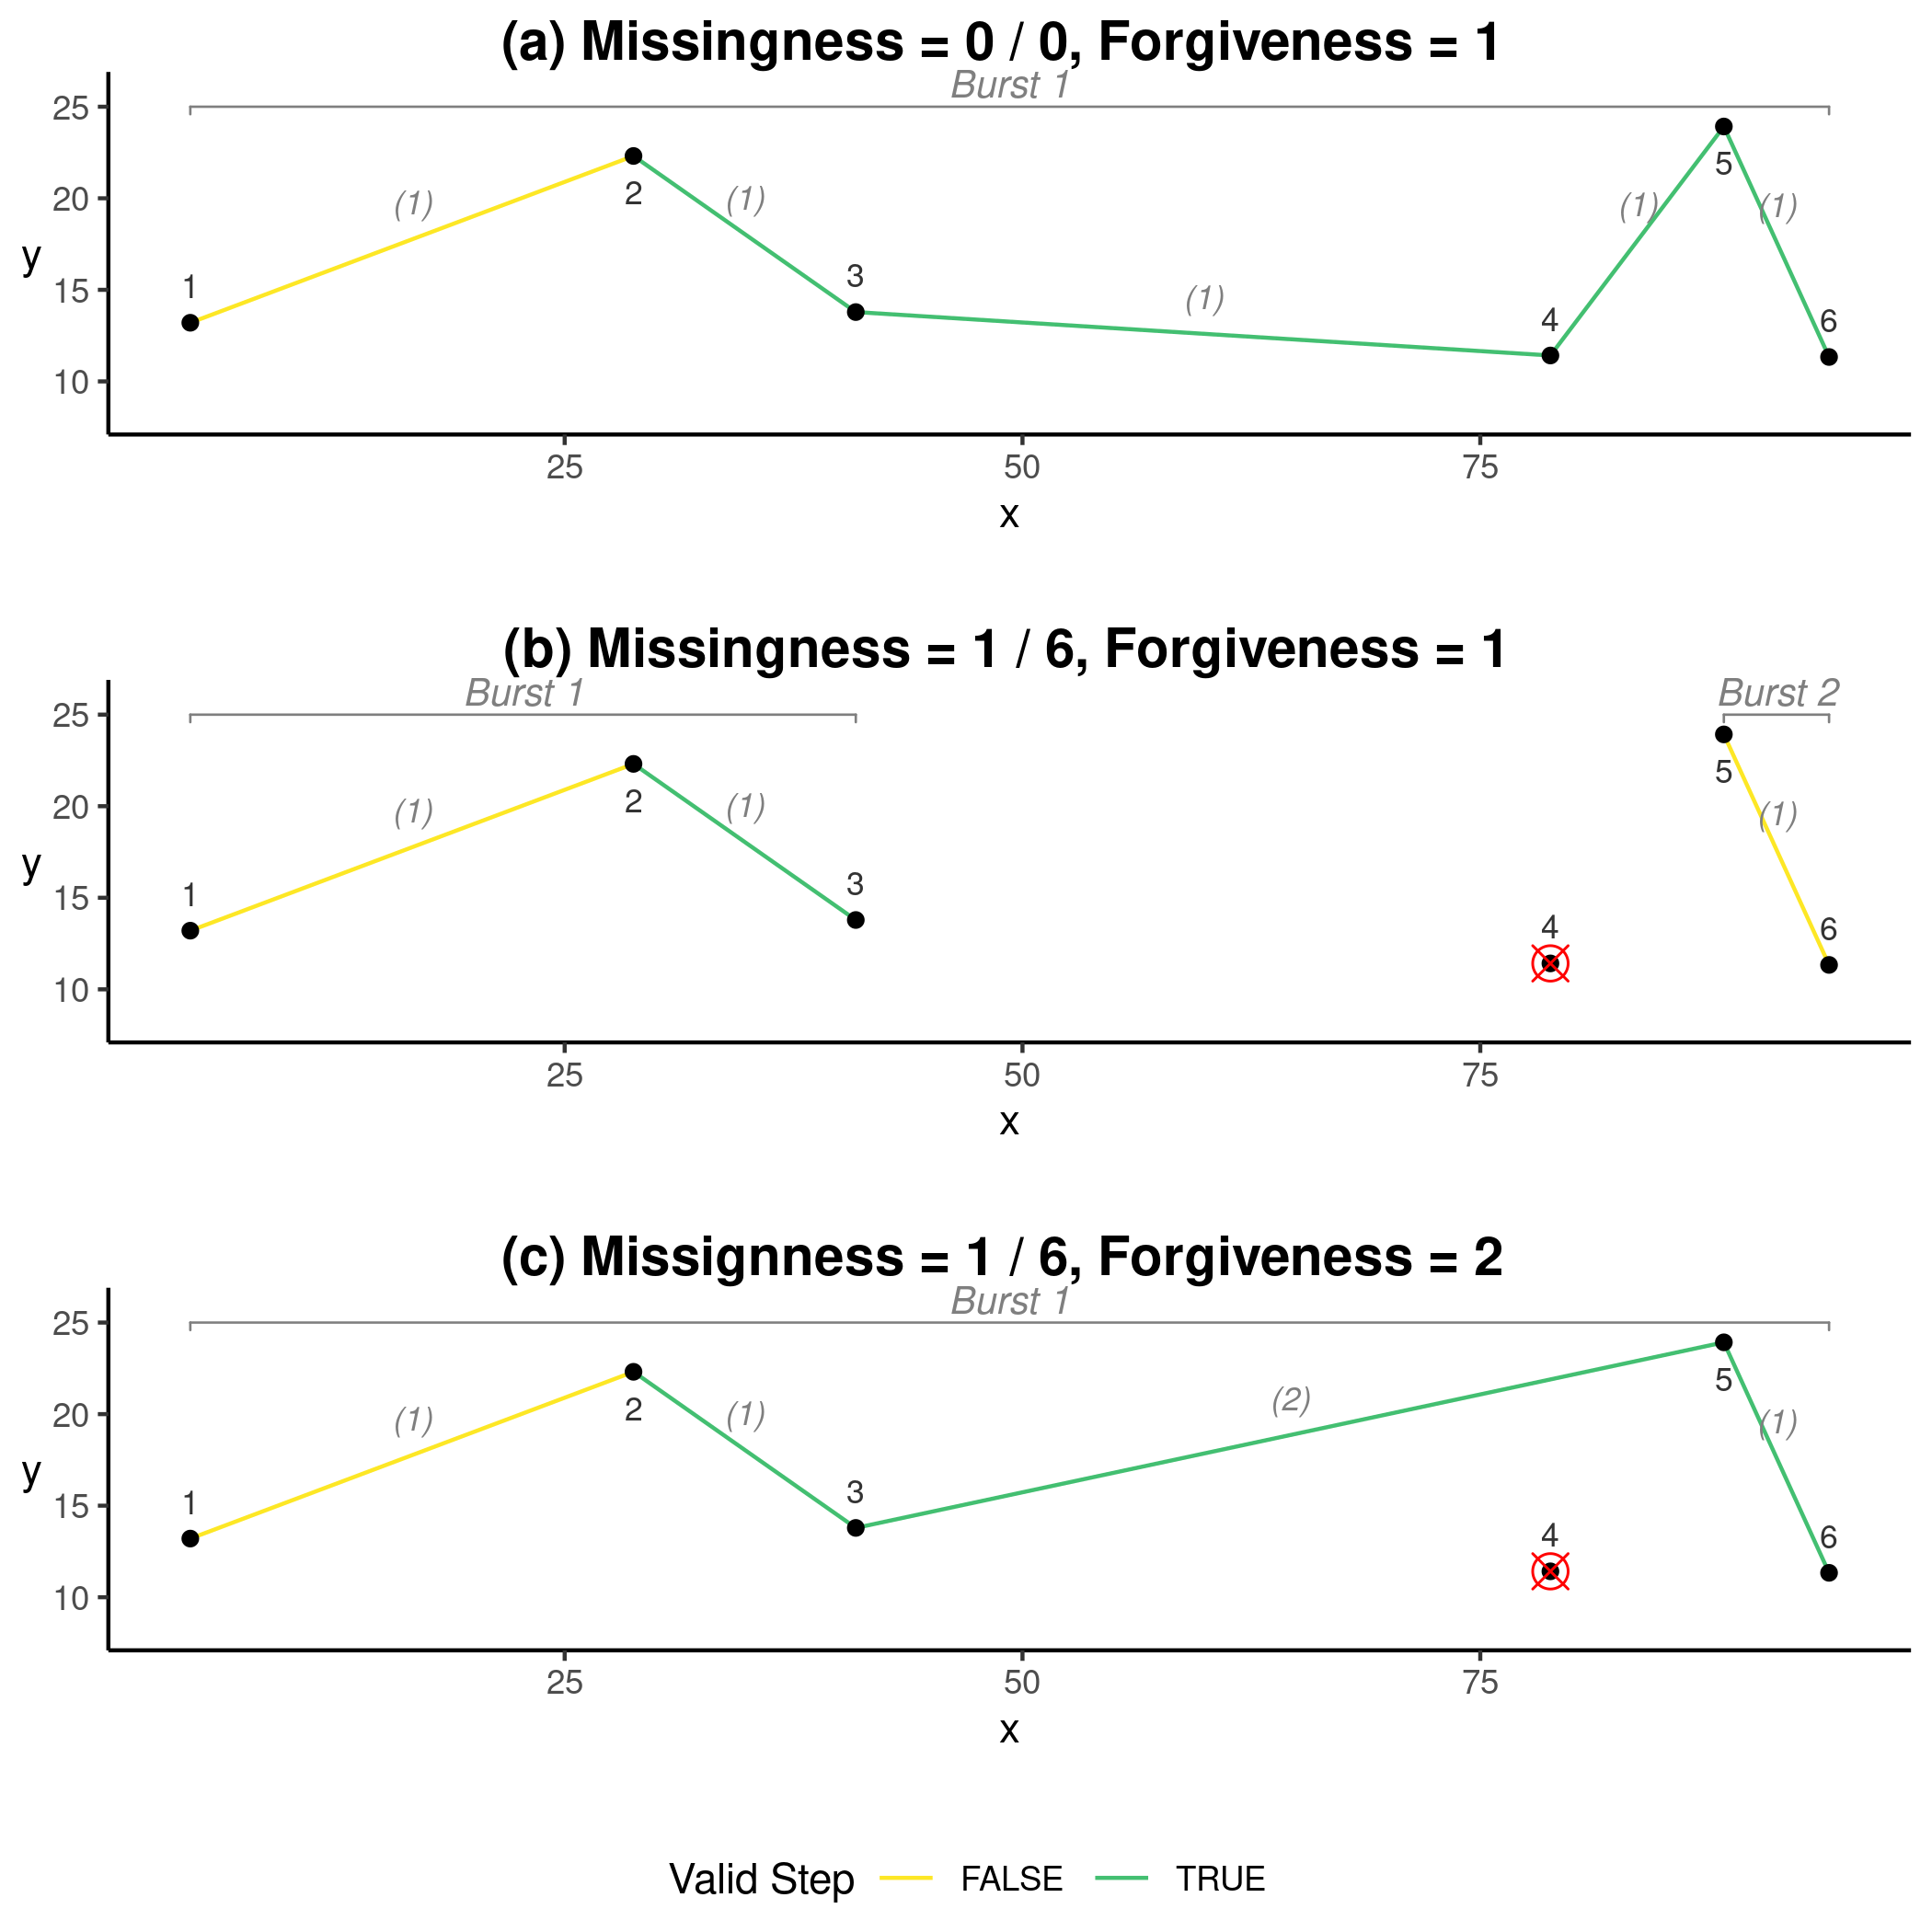
\includegraphics[width = \textwidth]{99_Overview.png}
  \caption{Figure demonstrating how a missing fix affects the number of valid
  steps that can be used for step selection analysis. In subfigure (a), a
  complete trajectory without any missing fixes is given. This trajectory
  results in a total of four valid steps that can be analysed (the first step is
  lacking a relative turning angle and thus invalid). Each of the steps in (a)
  has a step-duration of one, which is indicated in. In subfigure (b), the
  fourth fix was removed. If the modeler does excludes steps with step-durations
  above one (i.e. has a forgiveness of one), this results in only a single valid
  step for analysis. Finally, subfigure (c) depicts the same situation, yet with
  a modeler that has a forgiveness of two, and is thus willing to accept steps
  with a step-duration of two. Here, we end up with three valid steps.}
  \label{Overview}
  \end{center}
\end{figure}

Depending on the amount of available data and the number of missing GPS fixes,
only considering regular bursts might entail little sacrifice. In some
situations, however, removing irregular data will imply a substantial loss of
information. For instance, consider the trajectory depicted in \Cref{Overview}a.
Assuming that the fixes 1-5 were collected on a regular interval, this sequence
will result in 6 steps, 5 of which would be valid (for the first step we can't
compute a relative turning angle). If, however, the 4th fix is missing, and the
modeler is not willing to accept steps with a duration above one, then we are
down to a single valid step. That is, one missing fix reduced the number of
valid steps by three. If, on the other hand, the modeler deems a step-duration
of two as acceptable, we achieve three valid steps. From this example it is
clear that already a relatively small missingness implies a subsantial loss in
the number of valid steps that can be used for step selection analysis (see also
\Cref{ValidSteps}).

Additionally, recent developments in the SSA realm have brought
forward several improvements to SSA that might allow to relax the assumption of
regular step-durations. This includes the \textit{integrated} SSA approach
presented by \citep{Avgar.2016}, in which inference on habitat \textit{and}
movement preferences are possible thanks to the inclusion of movement
descriptors in the respective model. More recently, the method has been further
refined by \citep{Munden.2021}, who coined the term \textit{time-varying
integrated} SSA. This method was developed for high frequency data which has
been rarified using a change-point detection algorithm, thus also resulting in
irregular step-durations. In case of missing steps, in contrast, steps durations
are not entirely random but usually clustered.

Here, we questioned the practice of removing any irregular data in SSA and
investigated whether such data could be used to inform step selection models.
For this, we conducted a simulation study where we simulated movement
trajectories with known preferences across a virtual landscape. We then
artifically rarified the ``observed'' data by removing GPS fixes and we analysed
this data using SSA. This allowed us to investigate if and how the inclusion of
irregular data affected model estimates. We also varied the degree of
irregularity in the data and we tested for the effects of adjusting the
parametric step-length and turning distributions to different step-durations.
Besides the simulation study, we also analysed a dataset collected on dispersing
African wild dogs and examined the implications considering or discarding
irregular data.

Specifically, we employed six competing approaches to handle temporal
irregularity in the data.

\begin{figure}
  \begin{center}
  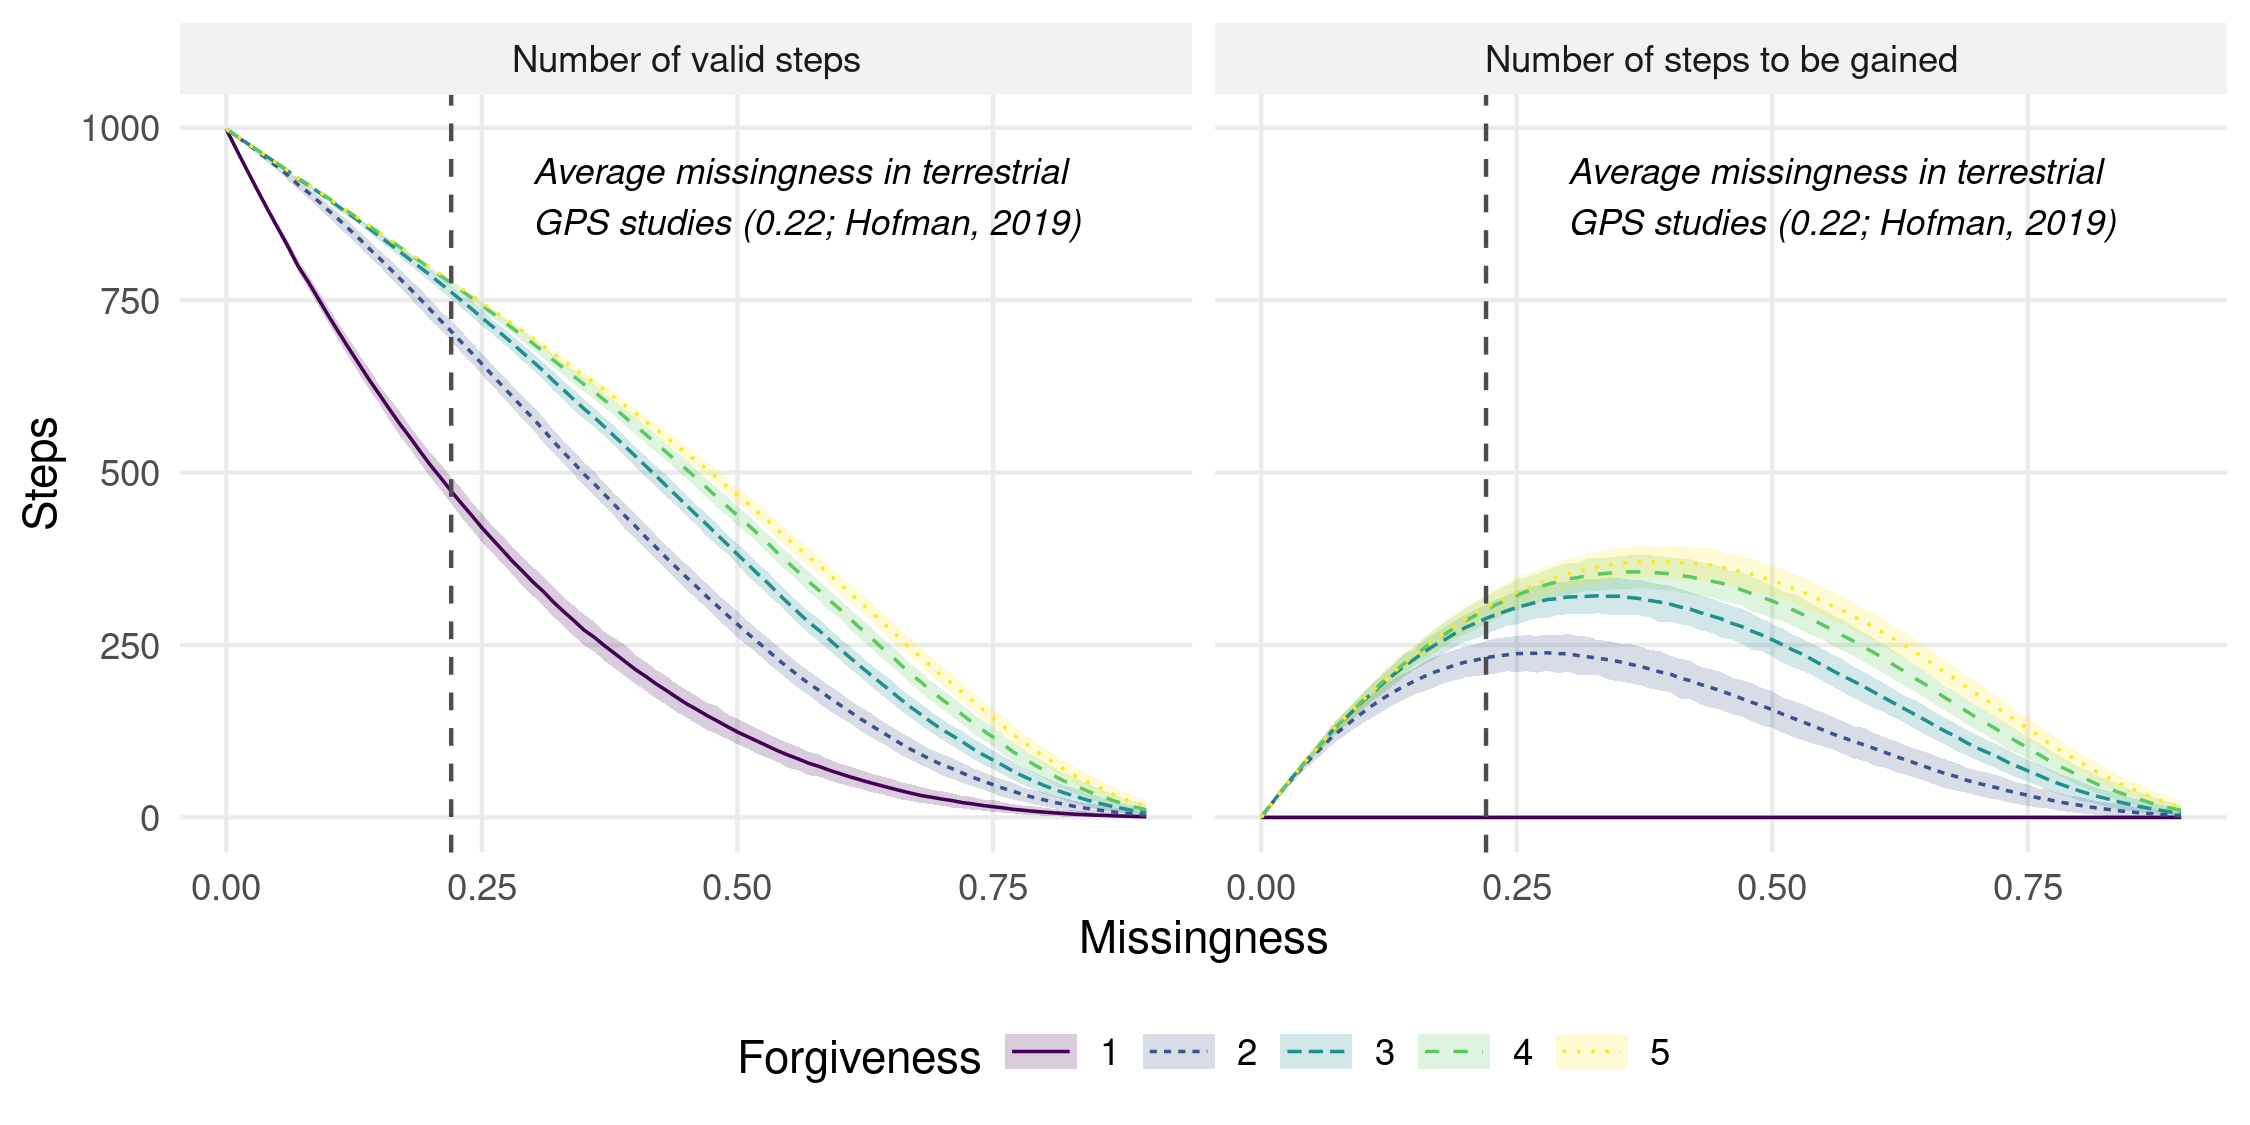
\includegraphics[width = \textwidth]{99_NumberOfSteps.png}
  \caption{Illustration of how missingness in GPS data reduces the number of
  steps that can be used in step selection analysis. At a missingness of 0, all
  1'000 theoretical GPS points could be used to compute steps, thus resulting in
  998 steps. However, if the missingness increases, data gaps will prevent the
  computation of some steps. However, the higher the forgiveness of a modeler,
  the more missing fixes a modeler will accept to still be able to compute a
  step.}
  \label{ValidSteps}
  \end{center}
\end{figure}

We hypothesized that the precision of model estimates would decrease as we
increased the missigngess in the data. We also expected that the inclusion of
irregular data would not improve the precision of estimates and rather lead to
biased values. However, we anticipated that such biases, at least in estimated
movement kernel parameters, could be reduced by appropriately adjusting the
availability domain.

\section{Methods}
\subsection{Spatial Covariates}
We simulated a virtual landscape comprising three spatial covariate layers, each
with a resolution of 300 x 300 pixels (\Cref{Covariates}) spanning across x- and
y-coordinates from 0 to 300. The first layer (\textsf{forest}) represented areas
covered by forest and was simulated using a random cluster nearest‐neighbour
neutral landscape model \citep{Saura.2000}, with the cluster-proportion set to
0.5 and the patch occupancy of forest fixed to 20\%. The second layer
(\textsf{elev}) resembled an elevation layer and was simulated using a Gaussian
random fields neutral landscape model \citep{Schlather.2015}, with an
autocorrelation range of 10, magnitude of variation of the landscape of 1, and a
magnitude of variation in scale of 0. We simulated both of these layers using
the r-package {\tt NLMR} \citep{Sciaini.2018}. The third layer (\textsf{dist})
indicated the distance (in pixels) to the center of the virtual landscape \((x =
150, y = 150)\), and can be understood as a point of attraction, such as, for
instance, the center of an animal's home-range. We computed spatial distances
using the r-package {\tt raster} \citep{Hijmans.2022}. We normalized the values
from all layers to a range between zero and one.

\begin{figure}
  \begin{center}
  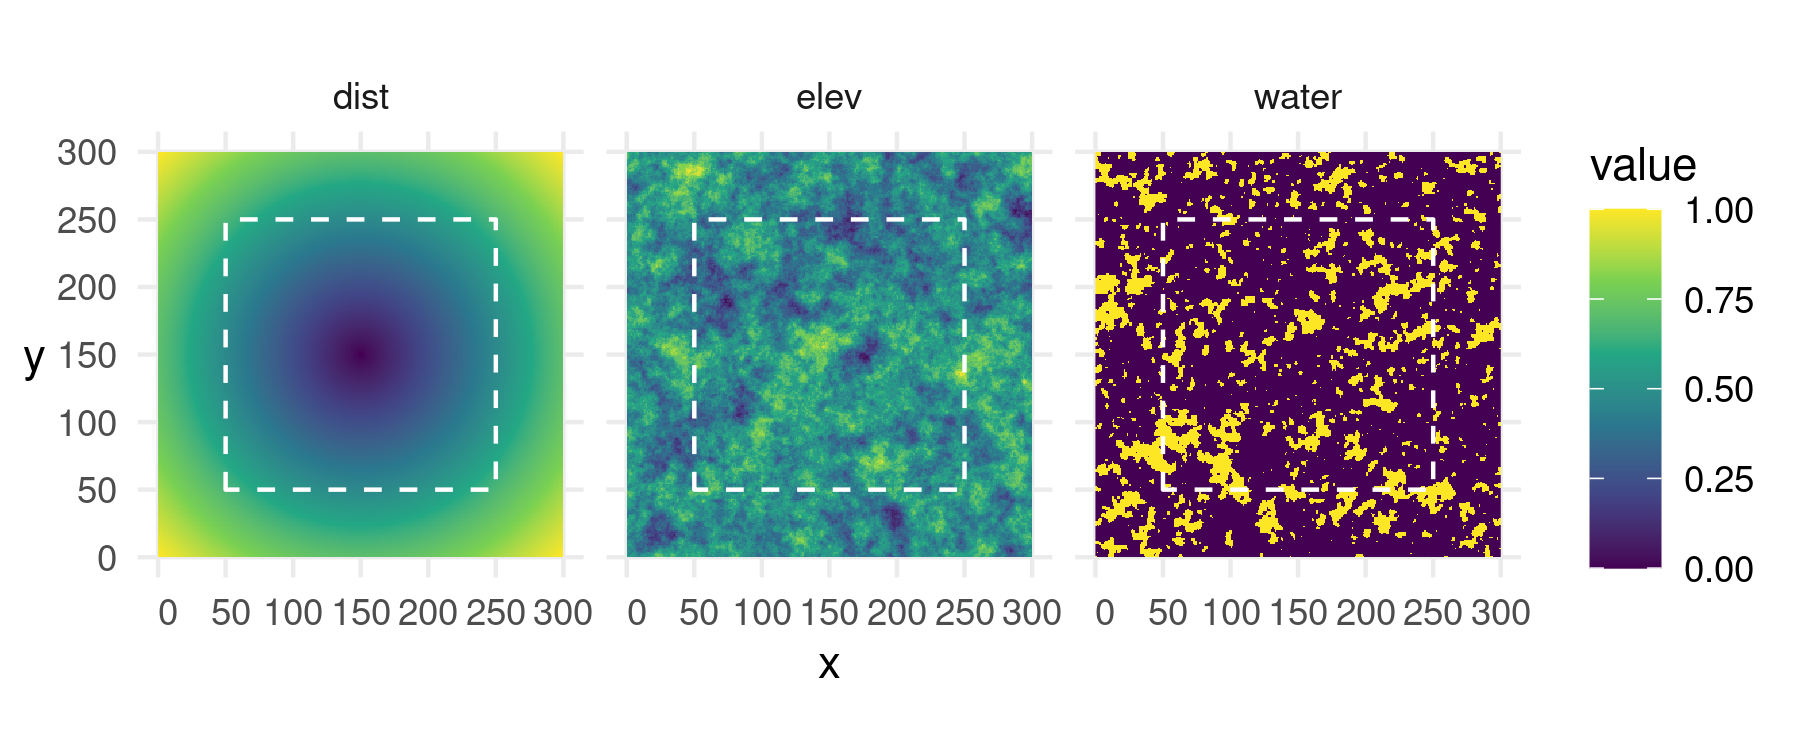
\includegraphics[width = \textwidth]{99_Covariates.png}
  \caption{Virtual landscape across which we simulated movement trajectories.
  All layers have a resolution of 300 x 300 pixels and were generated randomly.
  Simulated individuals were initiated within the white dashed rectangle, which
  ensured that they would not be released directly at a map border.}
  \label{Covariates}
  \end{center}
\end{figure}

\subsection{Movement Simulation}
To simulate movement across the virtual landscape, we employed an ``inverted''
step-selection function that proceeded as follows. First, we generated a random
starting location by sampling random x- and y-coordinates. To prevent starting
points in the vicinity of map borders, we restricted sampled locations to x- and
y-coordinates between 50 and 250 (white dotted rectangle in \Cref{Covariates}).
Second, we generated a set of 10 random steps originating from the randomly
selected starting point. We then generated random steps by sampling turning
angles from a von Mises distribution with concentration parameter \(\kappa =
0.5\) and location parameter \( \mu = 0 \), and step lengths from a gamma
distribution with shape parameter \(k = 3 \) and scale parameter \(\theta = 1\).
Third, we extracted covariate values along each random step from the underlying
covariate layers and computed the mean of each covariate along every step.
Fourth, we predicted for each step the probability of being chosen by applying
\Cref{EQ1}. The vector of relative selection strengths (i.e. the \(\beta\)s used
to make predictions was set to \(\beta_{forest} = -1\), \(\beta_{elev} = 0.5\),
and \(\beta_{dist} = -20\). Fifth, we sampled one of the random steps based on
predicted probabilities and computed the new position of the simulated
individual. We then repeated these steps until a total of 100 steps were. We
replicated the simulation 10'000 times, thus resulting in 10'000 independent
movement trajectories (\Cref{Simulations}). Although measurement error would
have been straight forward to implement, this was not the main focus of our
analysis and so we assumed GPS locations to be 100 percent accurate with regards
to an animal's true x- and y-locations. The simulated trajectories are depicted
in \Cref{Simulations}.

\begin{figure}
  \begin{center}
  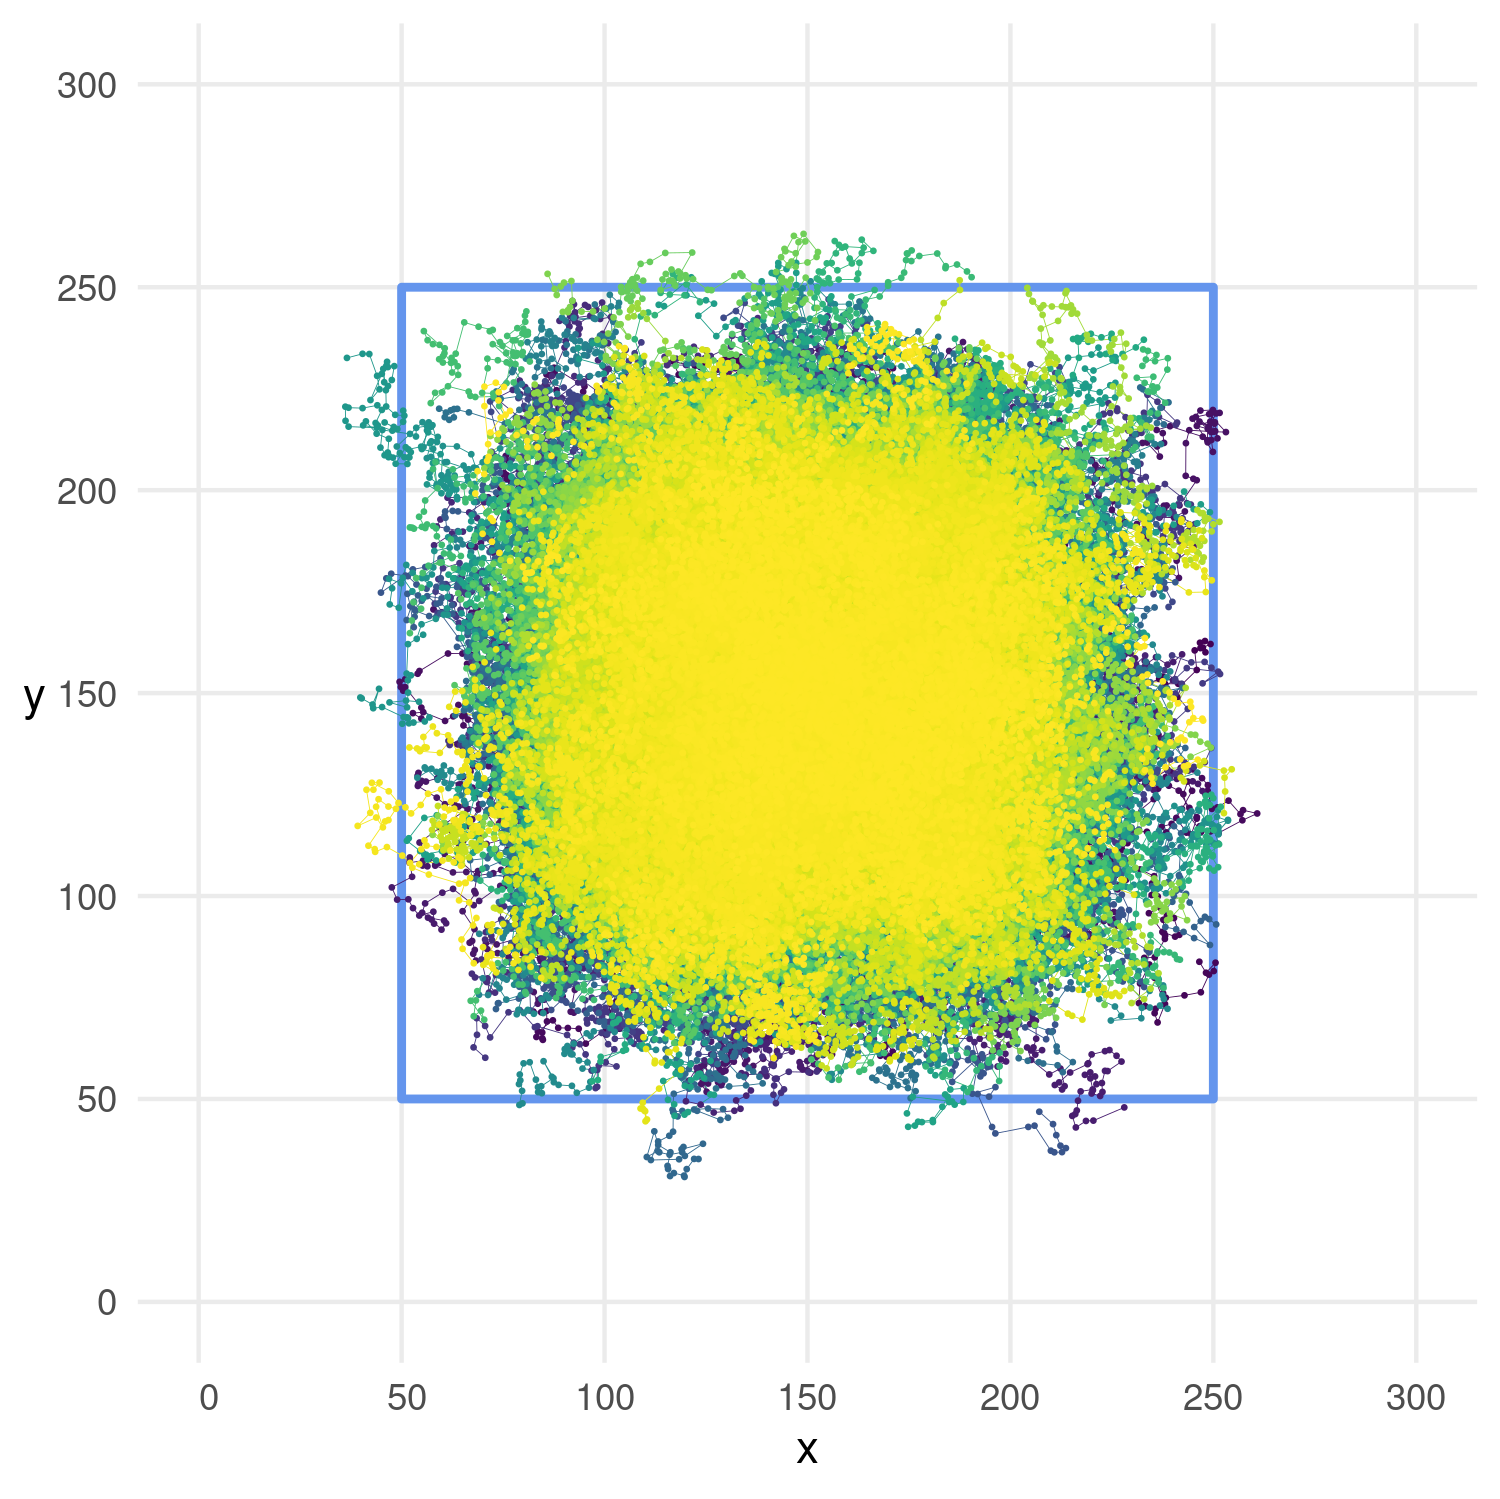
\includegraphics[width = 0.5\textwidth]{99_Simulations.png}
  \caption{10'000 Simulated movement trajectories, each comprising of 100 steps.
  Simulated individuals were initiated within the blue rectangle to mitigate
  edge effects.}
  \label{Simulations}
  \end{center}
\end{figure}

\subsection{Treatments}
To assess the consequences of missing GPS data in when employing step-selection
functions, we analysed the simulated GPS data under different conditions and
using different methods \Cref{Design}. Specifically, we varied the degree of
missingness (from 0\% to 50\%), the forgiveness with regard to step-durations
(from 1 to 5), and the way in which random steps were generated. We replicated
each treatment combination 100 times, estimated step-selection parameters and
computed averages and standard deviations for each treatment.

\subsection{Data Rarefication}
We rarefied the simulated GPS data by randomly removing a fixed fraction of GPS
fixes. To assess the impact of different degrees of ``missingness'', we varied
the fraction of removed data from 0 (complete dataset) to 0.5 (50\% missing)
with increments of 0.1. The random removal of GPS fixes introduced temporal
irregularity of the GPS fixes and so the resulting step-durations differed
depending on the time elapsed between remaining fixes. In the complete dataset,
a step-duration of one was assumed, whereas the step-duration increased by one
for every missing fix.

\subsection{Identifying Bursts and Computing Step Metrics}
We used the rarefied data to compute movement bursts. A movement burst consisted
of a sequence consecutive GPS fixes with step-durations that did not exceed the
forgiveness. For instance, if the forgiveness was one, already a single missing
GPS fix introduced a new burst. In contrast, if the forgiveness was two,
step-durations up to two were allowed without enforcing a new burst. For each
step in a burst we then computed the step length (\textsf{sl}), its natural
logarithm (\textsf{log(sl)}), and the cosine of the relative turning angle
(\textsf{cos(ta)}).

\subsection{Step Selection Function}
To conduct step selection analysis, we paired each observed step with 10 random
steps. In general, we generated random steps by sampling turning angles from a
von Mises distribution and step lengths from a gamma distribution, both fitted
to the observed data. However, depending on the chosen approach, the generation
of random steps differed slightly. Specifically, we employed six different
approaches:
\begin{itemize}
  \item \textit{Uncorrected}: In the \textit{uncorrected} approach, we sampled
  step-lengths and turning-angles from parametric distributions fitted to
  observed steps with step-durations of one. This approach ignores the fact that
  observed steps exhibit different step-durations.
  \item \textit{Na\"ive}: In the \textit{na\"ive} approach, we sampled
  step-lengths and turning-angles from parametric distributions fitted to
  observed steps with step-durations of one. However, we linearly scaled sampled
  step lengths to the step-duration of the observed step. For instance, for any
  step with a step-duration of two, we doubled sampled step lengths. This
  approach implicitly assumes that step lengths linearly scale with
  step-durations.
  \item \textit{Dynamic}: In the \textit{dynamic} approach, we sampled step
  lengths and turning angles from distributions that were fit to different
  step-durations. That is, for observed steps with step duration of two, we
  sampled step lengths and turning angles from distirbutions fit to observed
  steps of duration of two. To parametrize all the necessariy distributions, we
  randomly removed 50\% fixes from the simulated data and generated steps
  between the remaining fixes. This resulted in steps with varying
  step-durations. Based on the resulting step lengths and turning angles we
  fitted separate distributions for all step-durations. We replicated the
  subsampling procedure 1000 times and averaged the estimates for distribution
  parameters across replicates.
  \item \textit{Multistep}: In the \textit{multistep} approach, we sampled
  step-lengths and turning-angles from parametric distributions fitted to
  observed steps with step-durations of one. However, if an observed step had a
  step-durations larger than one, we augmented each random step with yet another
  random step. We repeated this augmentation until the number of consecutive
  steps matched the desired step-duration. For instance, for an observed step
  with step-duration of two, we sampled random steps twice and concatenated them
  into ``random paths''. The resulting paths were then simplified to a straight
  line connecting the first and last coordinate of each path.
  \item \textit{Model}: In the \textit{model} approach we sampled step lengths
  and turning angles from parametric distributions fitted to observed steps with
  step-durations of one. However, we accounted for potential differences in
  distribution parameters by including predictor variables in the model to
  update the distribution parameters depending on the step-duration (cfr
  \Cref{RegressionModel}).
  \item \textit{Imputed}: In the \textit{imputed} approach, we imputed missing
  fixes using predictions from a simple movement model. Specifically, we fitted
  fitted Johnson's single-state movement model \citep{Johnson.2008} to each
  observed trajectory and used the parameterized model to predict locations for
  the missing fixes. This resulted in a complete dataset without any missing
  fixes. We than sampled step-lengths and turning angles from distributions
  fitted to observed steps with step-duration of one.
\end{itemize}

Together, an observed and its 10 associated random steps formed a stratum that
received a unique ID. Along all steps we then extracted covariate values from
the underlying covariate layers and computed the mean of each covariate along
every step.

\begin{figure}
  \begin{center}
  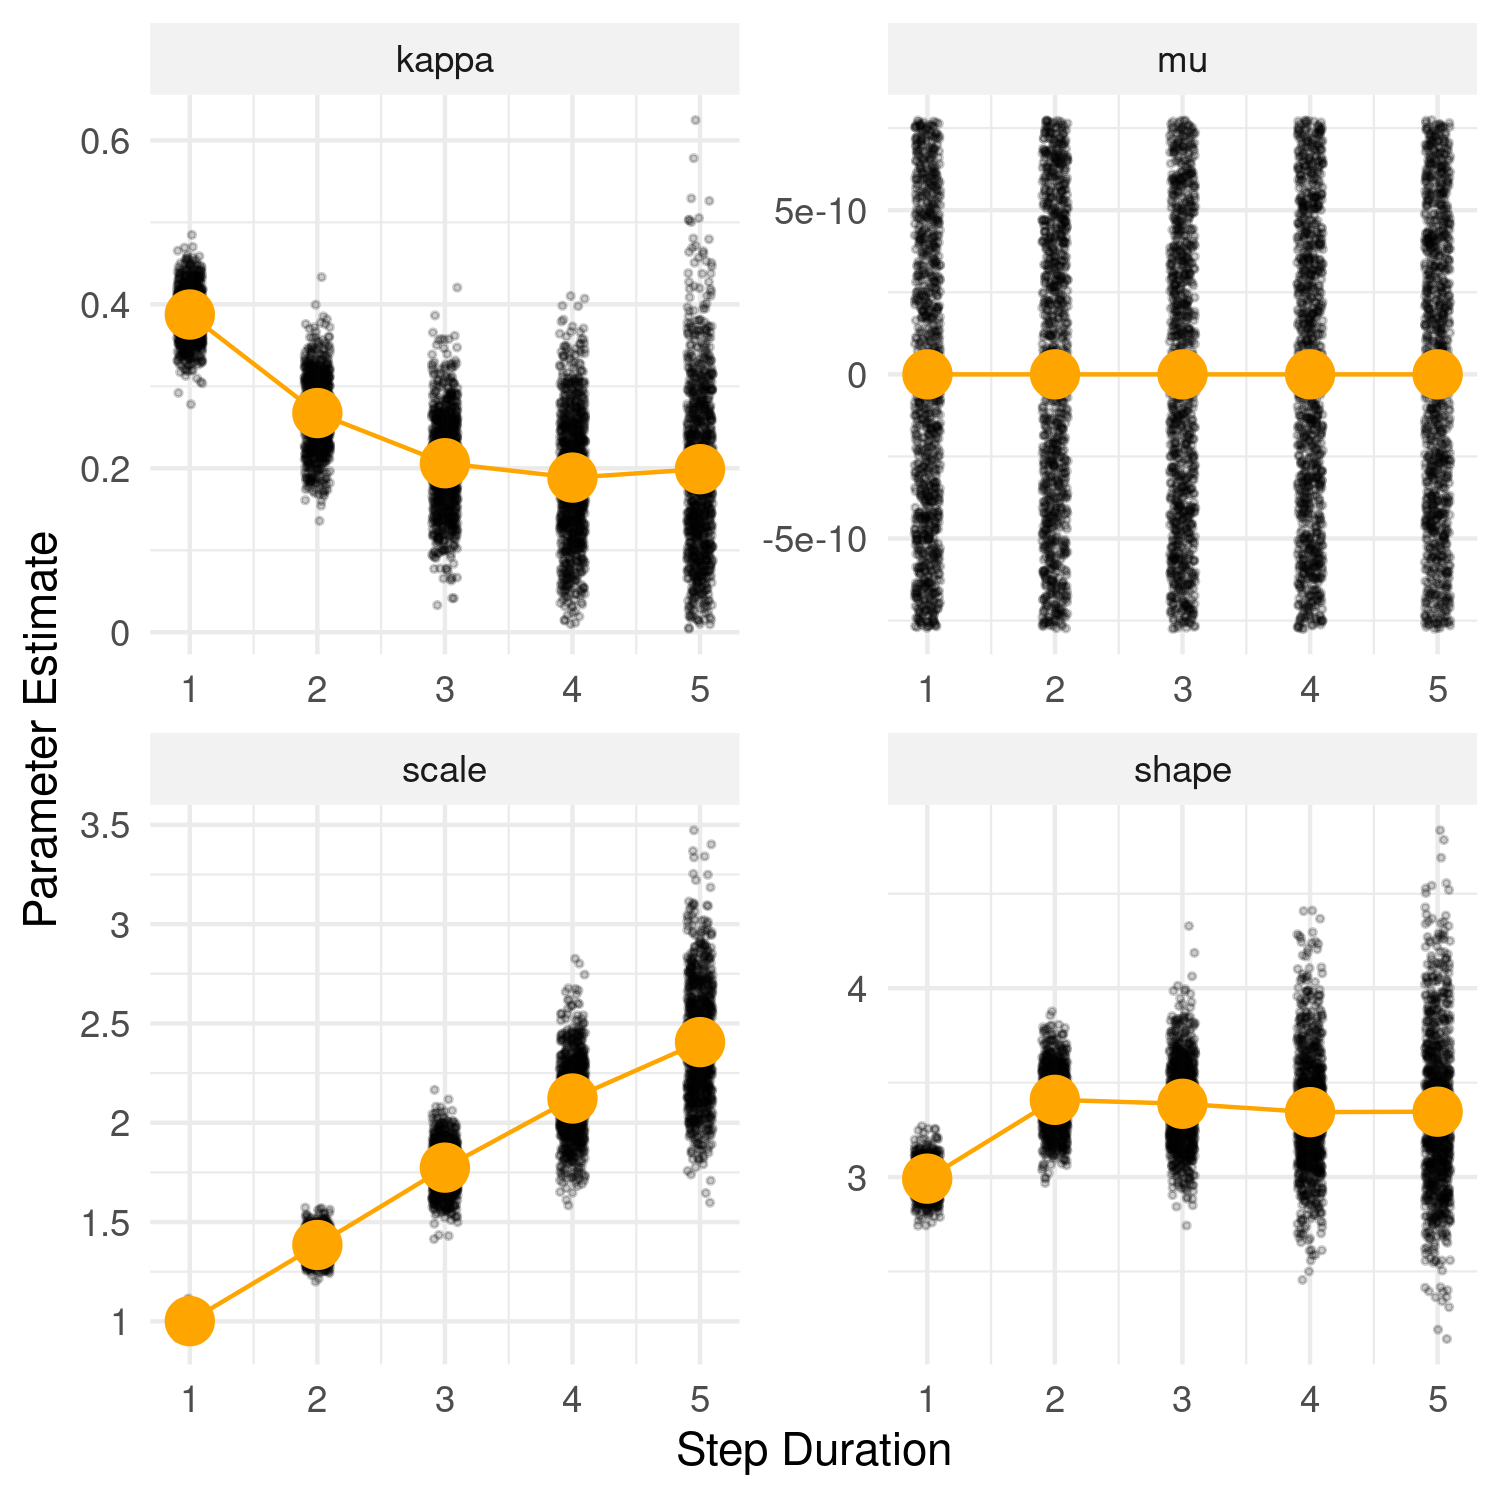
\includegraphics[width = \textwidth]{99_DistributionParameters.png}
  \caption{Parameter estimates for the von Mises distribution (top row) and
  gamma distribution (bottom row) fitted to steps with different durations. The
  von Mises distribution requires two parameters, namely a concentration
  parameter and a location parameter. Here, the conentration parameter
  diminishes as the step-duration increases, indicating that steps with higher
  step duration tend to be less directional. The location parameter, on the
  other hand, remains unchanged at 0, indicating that movement tends to be
  forward directed and is not biased towards left or right turns. The gamma
  distribution requires a shape and a scale parameter. Here, the shape parameter
  linearly increases with increasing step-duration, yet the shape parameter
  levels off at a step-duration of two.}
  \label{DistributionParameters}
  \end{center}
\end{figure}

\subsection{Regression Model}
\label{RegressionModel}
We estimated relative selection strengths (i.e. the \(\beta\)s in \Cref{EQ1})
using conditional logistic regression, implemented using the r-package
\textsf{survival} \citep{Therneau.2021}. That is, our response variable was a
binary variable indicating if a step was an observed (i.e. a case step, scored
1) or random step (i.e. a control step, scored 0). Following \cite{Avgar.2016}
and \cite{Fieberg.2021}, we employed \textit{integrated} SSA and besides habitat
covariates (\textsf{forest, elev, dist}), also included descriptors of the step
length and turning angle (\textsf{sl, log(sl), cos(ta)}) as predictors in our
regression model. Including those predictors allowed us to learn more about the
movement characteristics of the focal species and to update our tentative
parameters for the step-length and turning angle distirbutions (for further
details see \citealp{Fieberg.2021}). The model call was as follows:

$$
case \sim forest + elev + dist + sl + log(sl) + cos(ta)
$$

For the \textit{model} approach, however, the model call was slightly adjusted
and also included interactions between the factor covariate step-duration and
the movement descriptors. It thus looked as follows:

\begin{align*}
case \sim forest &+ elev + dist + sl + log(sl) + cos(ta) + sl:duration \\
  &+ log(sl):duration + cos(ta):duration
\end{align*}

We recorded beta estimates across all replicates, computed their means and
standard deviations for the different treatment combinations.

\section{Results}
\subsection{Habitat Kernel}

Model estimates for the habitat kernel are illustrated in \Cref{ResultsHabitat}.
\begin{figure}
  \begin{center}
  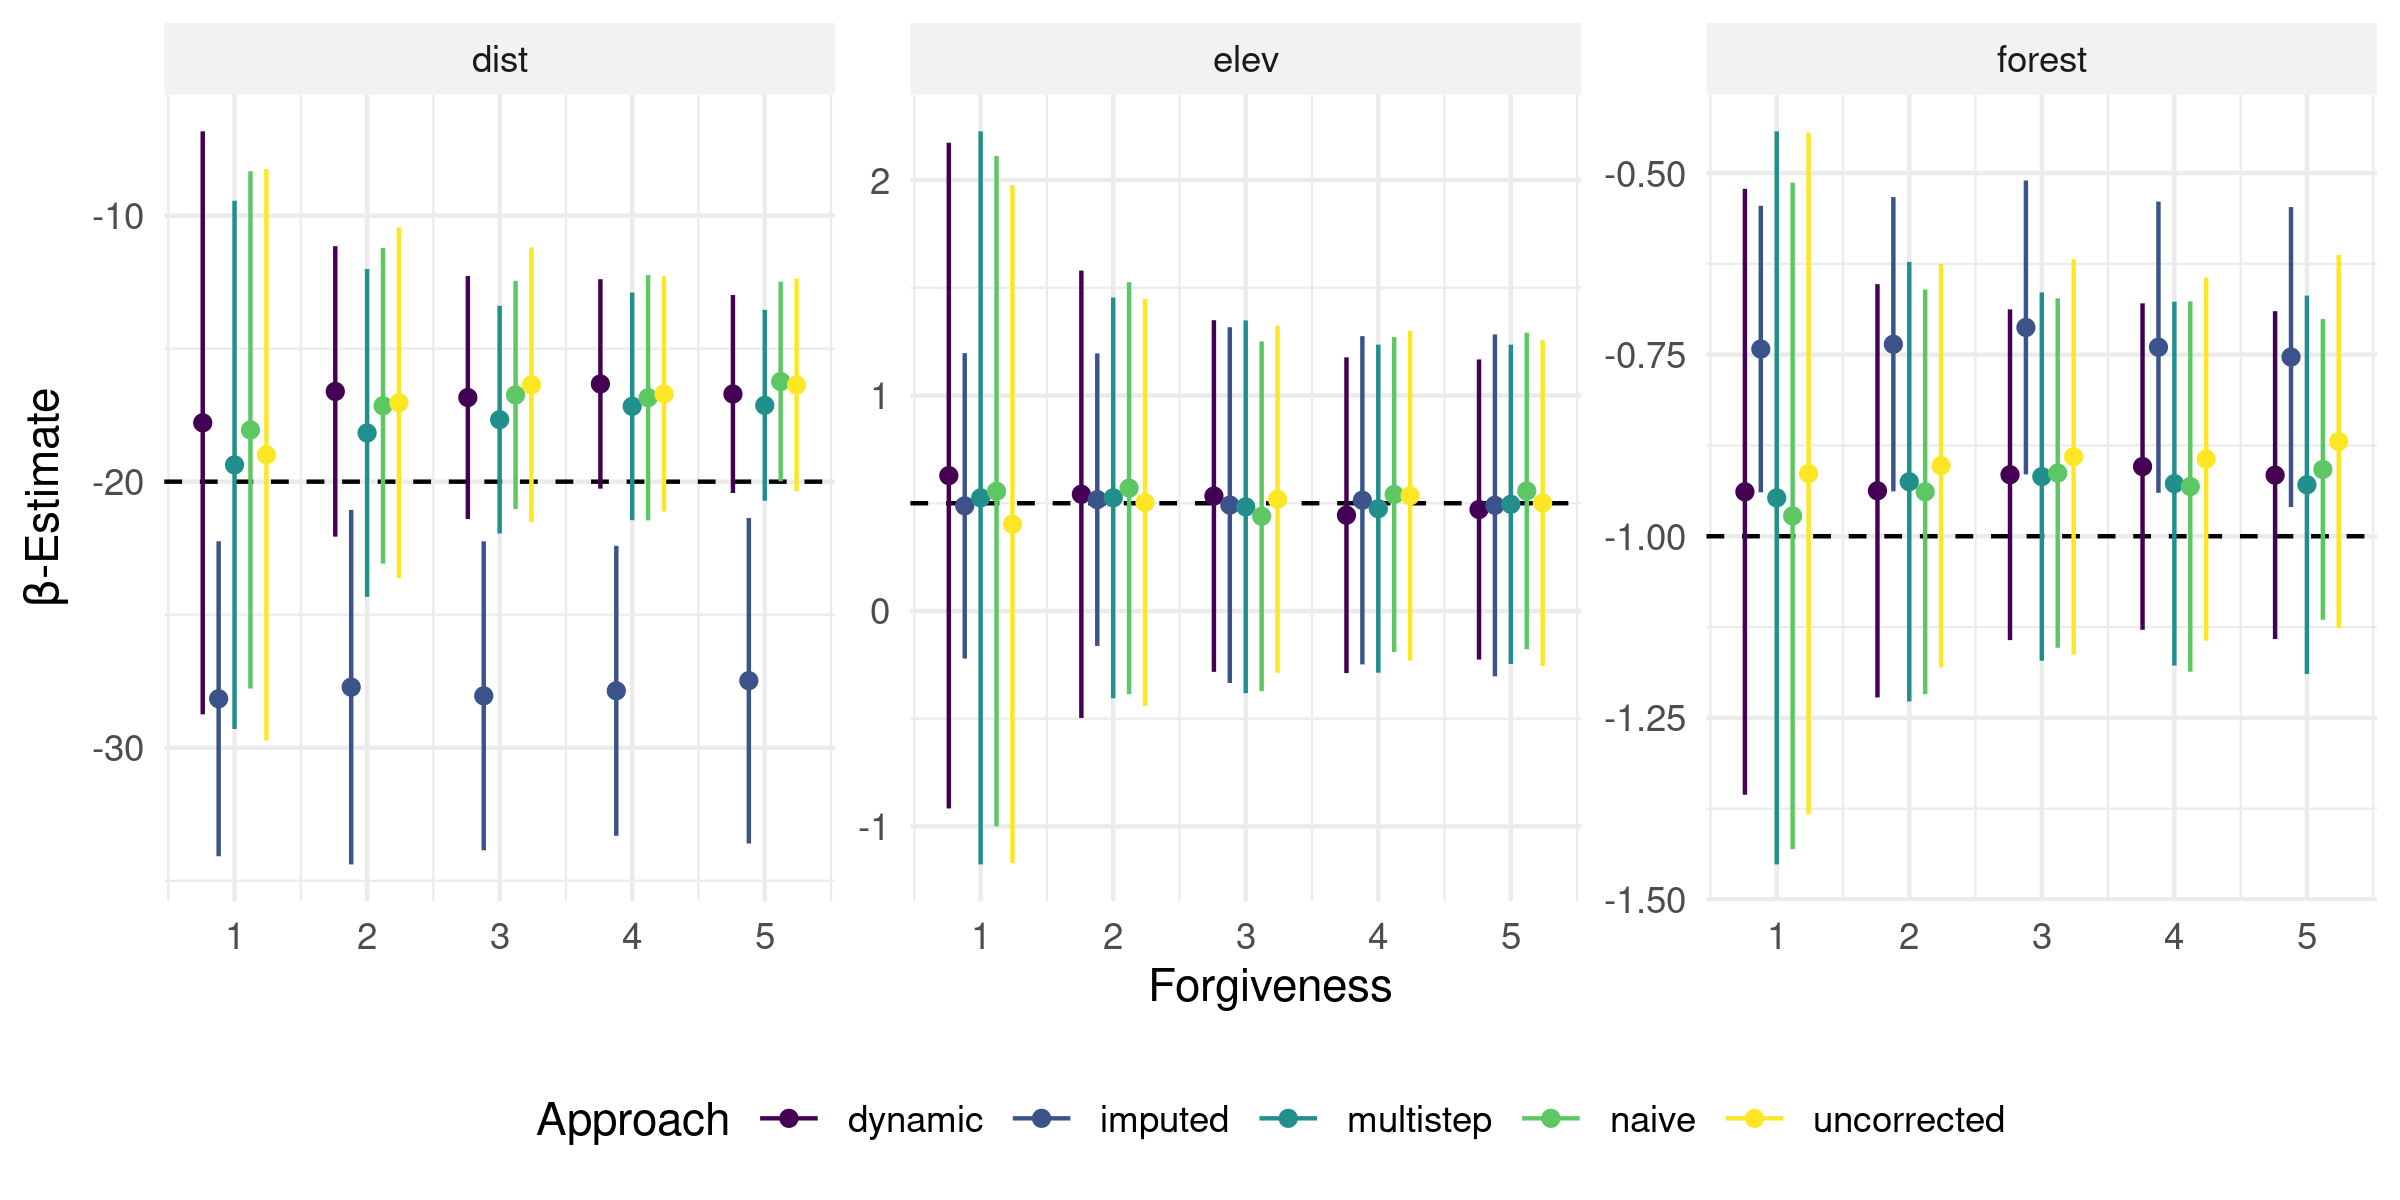
\includegraphics[width = \textwidth]{99_ResultsHabitatKernel.png}
  \caption{Parameter estimates with regards to the habitat covariates
  \textsf{dist}, \textsf{elev}, and \textsf{forest}. Dots indicate the mean
  estimates across 100 replicates, whereas the vertical line delineate $\pm 2SD$
  from the mean. The black dotted lines indicate the ``true'' values that were
  used to simulate movement. Colors separate different approaches to account for
  varying step-durations in the data. For clarity, we only show results for the
  treatments with data missingness of 0.5.}
  \label{ResultsHabitat}
  \end{center}
\end{figure}

\subsection{Movement Kernel}

\begin{figure}
  \begin{center}
  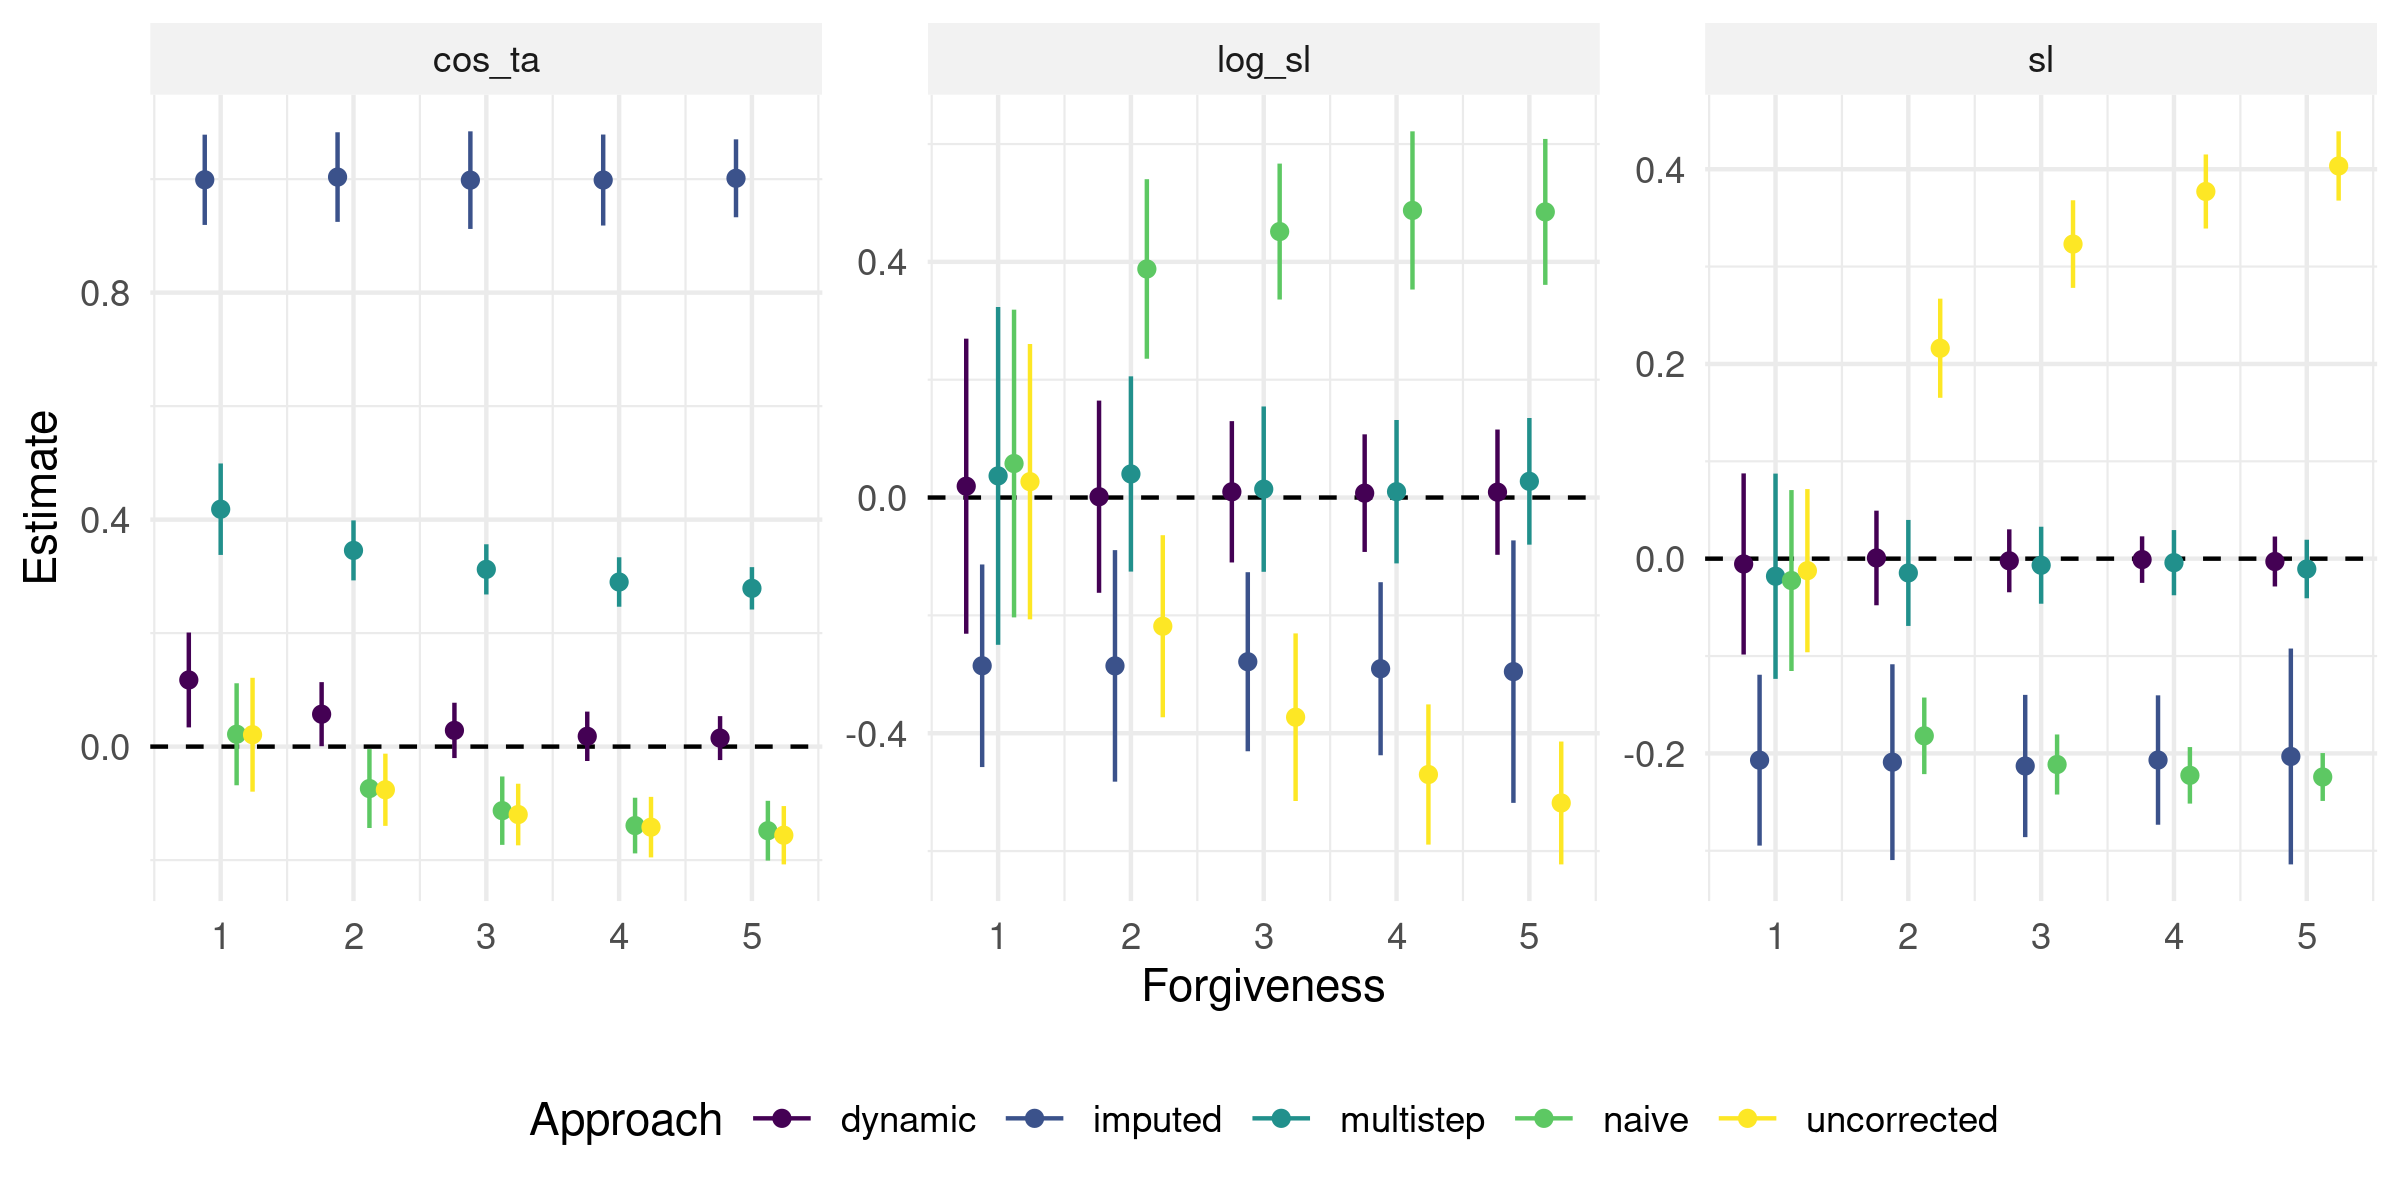
\includegraphics[width = \textwidth]{99_ResultsMovementKernel.png}
  \caption{Parameter estimates with regards to the movement covariates
  \textsf{sl}, \textsf{log(sl)}, and \textsf{cos(ta)}. Dots indicate the mean
  estimates across 100 replicates, whereas the vertical line delineate $\pm 2SD$
  from the mean. The black dotted lines indicate the ``true'' values that were
  used to simulate movement. Colors separate different approaches to account for
  varying step-durations in the data. For clarity, we only show results for the
  treatments with data missingness of 0.5.}
  \label{ResultsMovement}
  \end{center}
\end{figure}


\section{Discussion}
Results from our simulation study demonstrate that the inclusion of GPS fixes
can be used to gain information on relative habitat preferences of the focal
species. While the inclusion of steps from irregular sampling schemes resulted
in substantial biases for estimates related to step metrics, we showed that
these biases can effectively be mitigated by generating step lengths and turning
angles from distributions that are separately fit to steps from different step
durations. Regardless of biases in beta coefficients for step metrics, we found
that habitat selection estimates were unbiased, even when including irregular
steps. Even more, the inclusion of irregular steps drastially reduced model
uncertainty, thus suggesting that such data can be used to gain information that
would otherwise be lost.

\section{Authors' Contributions}
D.D.H., D.M.B., A.O. and G.C. conceived the study and designed methodology;
D.M.B., G.C., and J.W.M. collected the data; D.D.H. and D.M.B. analysed the
data; G.C. and A.O. assisted with modeling; D.D.H., D.M.B., and G.C. wrote the
first draft of the manuscript and all authors contributed to the drafts at
several stages and gave final approval for publication.

\section{Data Availability}
GPS movement data of dispersing wild dogs is available on dryad
\citep{Hofmann.2021b}. Access to R-scripts that exemplify the application of the
proposed approach using simulated data are provided through Github
(\url{https://github.com/DavidDHofmann/DispersalSimulation}). In addition, all
codes required to reproduce the African wild dog case study will be made
available through an online repository at the time of publication.

\section{Acknowledgements}
We thank the Ministry of Environment and Tourism of Botswana for granting
permission to conduct this research. We thank C. Botes, I. Clavadetscher, and G.
Camenisch for assisting with wild dog immobilizations. We also thank B. Abrahms
for sharing her data of three dispersing wild dogs. Furthermore, we would like
to thank Johannes Signer for assisting with the simulation algorithm. This study
was funded by Albert-Heim Foundation, Basler Stiftung für Biologische Forschung,
Claraz Foundation, Idea Wild, Jacot Foundation, National Geographic Society,
Parrotia Stiftung, Stiftung Temperatio, Wilderness Wildlife Trust Foundation,
Forschungkredit der Universität Zürich, and a Swiss National Science Foundation
Grant (31003A\_182286) to A. Ozgul.

\newpage
\begingroup
\singlespacing
\bibliography{Literatur}
\endgroup

\end{document}
